\documentclass[a4paper,12pt]{article}

\usepackage{float}


\usepackage[utf8]{inputenc}
\usepackage[dvips]{graphicx}
%\usepackage{a4wide}
\usepackage{epsfig}
\usepackage{fancybox}
\usepackage{verbatim}
\usepackage{array}
\usepackage{latexsym}
\usepackage{alltt}
\usepackage{amssymb}
\usepackage{amsmath,amsthm}
\usepackage{bm}
\usepackage{wasysym}

%\usepackage{fullpage}
%\usepackage{hyperref}
\usepackage{listings}
\usepackage{color}
\usepackage{algorithm}
\usepackage{algpseudocode}
\usepackage[hmargin=2cm,vmargin=3.0cm]{geometry}
%\topmargin=0cm
%\topmargin=-1.8cm
%\addtolength{\textheight}{6.5cm}
%\addtolength{\textwidth}{2.0cm}
%\setlength{\leftmargin}{-3cm}
%\setlength{\oddsidemargin}{0.0cm}
%\setlength{\evensidemargin}{0.0cm}

%misc libraries goes here
\usepackage{tikz}
\usepackage{tikz-qtree}
\usetikzlibrary{automata,positioning}

\usepackage{multicol}
\usepackage{enumitem}

\usepackage[most]{tcolorbox}

\usepackage[colorlinks=true,urlcolor=black,linkcolor=black]{hyperref}


\lstdefinestyle{customtex}{
    %backgroundcolor=\color{lbcolor},
    tabsize=2,
    language=TeX,
    numbers=none,
    basicstyle=\footnotesize\ttfamily,
    numberstyle=\footnotesize,
    aboveskip={0.0\baselineskip},
    belowskip={0.0\baselineskip},
    %
    columns=flexible,
    keepspaces=true,
    fontadjust=true,
    upquote=true,
    %
    breaklines=true,
    prebreak=\raisebox{0ex}[0ex][0ex]{\ensuremath{\hookleftarrow}},
    frame=single,
    showtabs=false,
    showspaces=false,
    showstringspaces=false,
    %
    %identifierstyle=\color[rgb]{0,0.2,0.8},
    identifierstyle=\color[rgb]{0,0,0.5},
    %identifierstyle=\color[rgb]{0.133,0.545,0.133},
    %keywordstyle=\color[rgb]{0.8,0,0},
    %keywordstyle=\color[rgb]{0.133,0.545,0.133},
    keywordstyle=\color[rgb]{0,0,0.5},
    %commentstyle=\color[rgb]{0.133,0.545,0.133},
    commentstyle=\color[rgb]{0.545,0.545,0.545},
    %stringstyle=\color[rgb]{0.827,0.627,0.133},
    stringstyle=\color[rgb]{0.133,0.545,0.133},
    %
    literate={â}{{\^{a}}}1 {Â}{{\^{A}}}1 {ç}{{\c{c}}}1 {Ç}{{\c{C}}}1 {ğ}{{\u{g}}}1 {Ğ}{{\u{G}}}1 {ı}{{\i}}1 {İ}{{\.{I}}}1   {ö}{{\"o}}1 {Ö}{{\"O}}1 {ş}{{\c{s}}}1 {Ş}{{\c{S}}}1 {ü}{{\"u}}1 {Ü}{{\"U}}1 {~}{$\sim$}{1}
}

\lstdefinestyle{output}{
    %backgroundcolor=\color{lbcolor},
    tabsize=2,
    numbers=none,
    basicstyle=\footnotesize\ttfamily,
    numberstyle=\footnotesize,
    aboveskip={0.0\baselineskip},
    belowskip={0.0\baselineskip},
    %
    columns=flexible,
    keepspaces=true,
    fontadjust=true,
    upquote=true,
    %
    breaklines=true,
    prebreak=\raisebox{0ex}[0ex][0ex]{\ensuremath{\hookleftarrow}},
    frame=single,
    showtabs=false,
    showspaces=false,
    showstringspaces=false,
    %
    %identifierstyle=\color[rgb]{0.44,0.12,0.1},
    identifierstyle=\color[rgb]{0,0,0},
    keywordstyle=\color[rgb]{0,0,0},
    commentstyle=\color[rgb]{0,0,0},
    stringstyle=\color[rgb]{0,0,0},
    %
    literate={â}{{\^{a}}}1 {Â}{{\^{A}}}1 {ç}{{\c{c}}}1 {Ç}{{\c{C}}}1 {ğ}{{\u{g}}}1 {Ğ}{{\u{G}}}1 {ı}{{\i}}1 {İ}{{\.{I}}}1   {ö}{{\"o}}1 {Ö}{{\"O}}1 {ş}{{\c{s}}}1 {Ş}{{\c{S}}}1 {ü}{{\"u}}1 {Ü}{{\"U}}1
}

\lstset{style=customtex}


\tikzset{%
    terminal/.style={draw, rectangle,
    				 align=center, 
					 minimum height=1cm, 
					 minimum width=2cm,
					 fill=black!10,
					 anchor=mid},
    nonterminal/.style={draw, rectangle,
    					align=left,
					    minimum height=1cm, 
						minimum width=2cm, 
						anchor=mid},% and so on
}

%% Style for terminals
%\tikzstyle{terminal}=[draw, rectangle, 
%					  minimum height=1cm, 
%					  minimum width=2cm, 
%					  fill=black!20,
%					  anchor=south west]
%% Style for nonterminals
%\tikzstyle{nonterminal}=[draw, rectangle, 
%						 minimum height=1 cm, 
%						 minimum width=2 cm, 
%						 anchor=north east]


\newcommand{\HRule}{\rule{\linewidth}{1mm}}
\newcommand{\kutu}[2]{\framebox[#1mm]{\rule[-2mm]{0mm}{#2mm}}}
\newcommand{\gap}{ \\[1mm] }

\newcommand{\Q}{\raisebox{1.7pt}{$\scriptstyle\bigcirc$}}
\newcommand{\minus}{\scalebox{0.35}[1.0]{$-$}}

\setlength{\fboxsep}{10pt}

\tcbsetforeverylayer{enhanced jigsaw, breakable, arc=0mm, boxrule=1pt, boxsep=5pt, after=\vspace{1em}, colback=white, colframe=black}

\newcolumntype{P}[1]{>{\centering\arraybackslash}p{#1}}

\setlength\parindent{0pt}

%\renewcommand\arraystretch{1.2}

\newenvironment{Tab}[1]
  {\def\arraystretch{1}\tabular{#1}}
  {\endtabular}

%%%%%%%%%%%%%%%%%%%%%%%%%%%%%%%%%%%%%%%%%%%%%%%%%%%%%%%%%%%%%%%%%%%%%%%%%%%%%%%%%%%%%%

\title{Formal Languages and Abstract Machines \\ Take Home Exam 2}
\author{Alper KOCAMAN \\ 2169589} % write your name and id
\date{} % do not write any date

%%%%%%%%%%%%%%%%%%%%%%%%%%%%%%%%%%%%%%%%%%%%%%%%%%%%%%%%%%%%%%%%%%%%%%%%%%%%%%%%%%%%%%

\begin{document}
\HRule\\
Middle East Technical University \hfill Department of Computer Engineering
{\let\newpage\relax\maketitle}
\HRule\\
\vspace{1cm}

%%%%%%%%%%%%%%%%%%%%%%%%%%%%%%%%%%%%%%%%%%%%%%%%%%%%%%%%%%%%%%%%%%%%%%%%%%%%%%%%%%%%%%

% Write your answers below the section tags
\section{Context-Free Grammars \hfill \normalfont{(10 pts)}}

\paragraph{a)} Give the rules of the Context-Free Grammars to recognize strings in the given languages where $\Sigma=\{a,b\}$ and $S$ is the start symbol. \\  

$L(G)=\{w \mid \;  w \in \Sigma^*;\; |w| \geq 3;\; $  \hfill \small{(2/10 pts)} \\
\hspace*{22mm} the first and the second from the last symbols of $w$ are the same$\}$ \\

\begin{tcolorbox}

$S \to aMab|aMaa|bMba|bMbb$\\\\
$M \to aM|bM|MM|\varepsilon$\\

\end{tcolorbox}


$L(G)=\{w \mid \;  w \in \Sigma^*;\; $ the length of w is odd$\}$ \hfill \small{(2/10 pts)} \\

\begin{tcolorbox}

$S \to aM|bM$\\\\
$M \to aMa|aMb|bMa|bMb|\varepsilon$\\

\end{tcolorbox}


$L(G)=\{w \mid \;  w \in \Sigma^*;\; n(w,a)=2\cdot n(w,b)\}$ where $n(w,x)$ is the number of $x$ symbols in $w$ \hfill \small{(3/10 pts)} \\

\begin{tcolorbox}

$S \to aSaSbS|aSbSaS|bSaSaS|\varepsilon$\\

\end{tcolorbox}



\paragraph{b)} Find the set of strings recognized by the CFG rules given below:         \hfill \small{(3/10 pts)} \\


$S \to X \mid Y$ \\
$X \to aXb \mid A \mid B$ \\
$A \to aA \mid a$ \\
$B \to Bb \mid b$ \\
$Y \to CbaC$ \\
$C \to CC \mid a \mid b \mid \varepsilon$  \\

\begin{tcolorbox}
S can select X or Y.\\
If X is chosen,then recognized string in that form:\\
First 0 or more a's are in the string,then 0 or more b's come but number of a's and number of b's cannot be equal.\\
Formally,let the set of recognized string be X,than set $X=\{(a^*b^*) \backslash (a^nb^n):n\geq 1\} \cup \{a\} \cup \{b\}$ or $X=\{(a^nb^m):n\geq 0,m\geq 0, n \neq m \}$.\\\\
Y can also be selected.\\
If Y is chosen,then recognized string in that form:\\
The string contains at least 1 'b' and after that 'b',at least 1 'a',namely this string contains 'ba' as a substring.\\
Formally,let the set of recognized string be Y,than set $Y=\{(a^*b^*)(ba) (a^*b^*)\}$.\\\\
Thus,the recognized set of strings are $X\cup Y$.\\
$X\cup Y=\{(a^nb^m):n\geq 0,m\geq 0, n \neq m \} \cup \{(a^*b^*)(ba) (a^*b^*)\}$ 

\end{tcolorbox}


\newpage
\section{Parse Trees and Derivations \hfill \normalfont{(20 pts)}}
Given the CFG below, provide parse trees for given sentences in \textbf{a} and \textbf{b}.\\

\begin{lstlisting}[style=output,mathescape=true]
S   $\to$ NP VP
VP  $\to$ V NP | V NP PP
PP  $\to$ P NP
NP  $\to$ N | D N | NP PP
V   $\to$ wrote | built | constructed
D   $\to$ a | an | the | my
N   $\to$ John | Mary | Jane | man | book | automata | pen | class
P   $\to$ in | on | by | with
\end{lstlisting}

\paragraph{a)} Jane constructed automata with a pen \hfill \small{(4/20 pts)} \\

\begin{tcolorbox}

\begin{center}

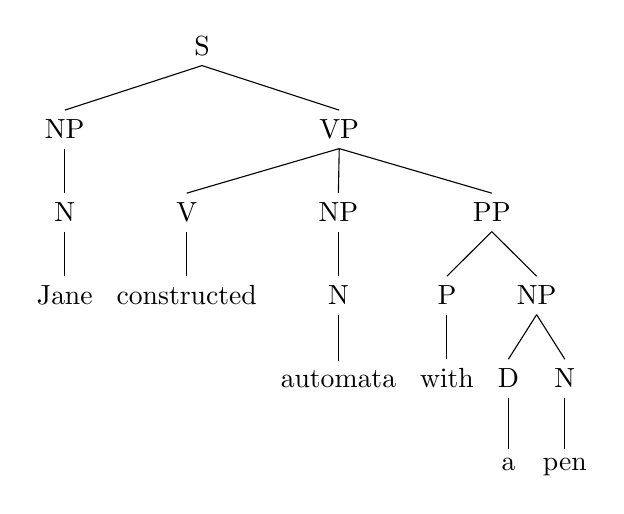
\begin{tikzpicture}[scale=1]
\Tree [.S [.NP [.N $$Jane$$ ] ][.VP [.V constructed ] [.NP [.N $$automata$$ ] ] [.PP [.P $$with$$ ] [.NP [.D $$a$$ ] [.N $$pen$$ ] ] ] ] ]
\end{tikzpicture}

\end{center}

\begin{center}

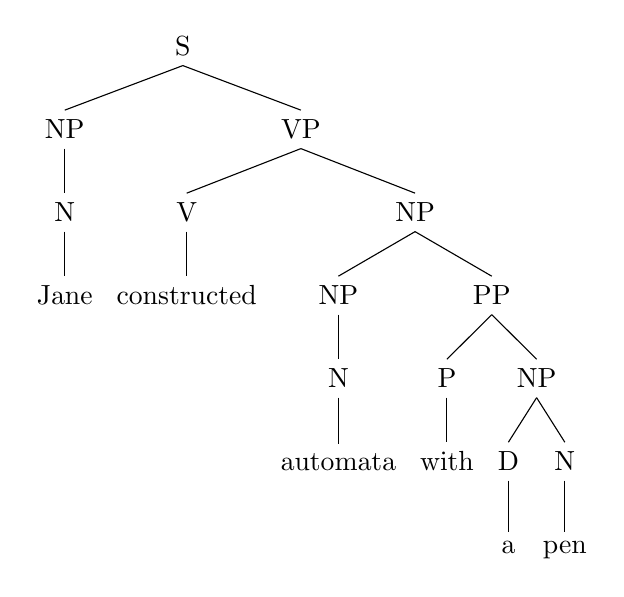
\begin{tikzpicture}[scale=1]
\Tree [.S [.NP [.N $$Jane$$ ] ][.VP [.V constructed ][.NP [.NP [.N $$automata$$ ] ] [.PP [.P $$with$$ ] [.NP [.D $$a$$ ] [.N $$pen$$ ] ] ] ] ] ]
\end{tikzpicture}

\end{center}

\end{tcolorbox}

\newpage

\paragraph{b)} my book in the man built a Jane by a pen \hfill \small{(4/20 pts)} \\

\begin{tcolorbox}
\begin{center}

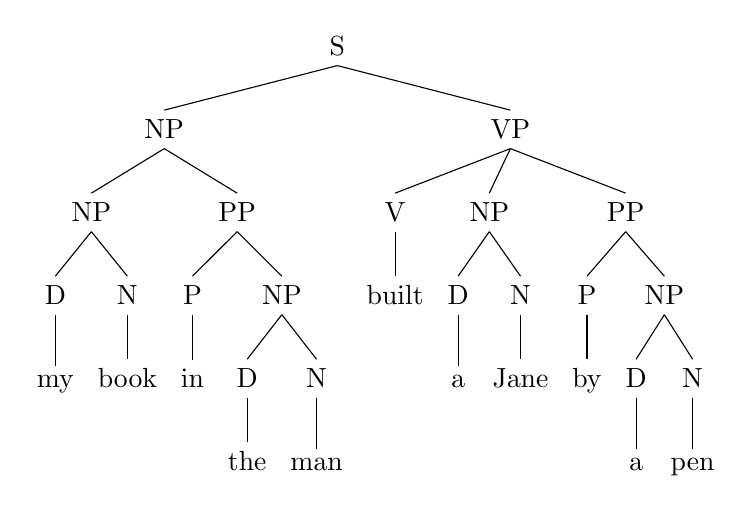
\begin{tikzpicture}[scale=1]
\Tree [.S [.NP [.NP [.D $$my$$ ] [.N $$book$$ ] ] [.PP [.P $$in$$ ] [.NP [.D $$the$$ ] [.N $$man$$ ]]] ][.VP [.V built ] [.NP [.D $$a$$ ] [.N $$Jane$$  ] ] [.PP [.P $$by$$ ] [.NP [.D $$a$$ ] [.N $$pen$$ ] ] ] ] ]
\end{tikzpicture}

\end{center}

\begin{center}

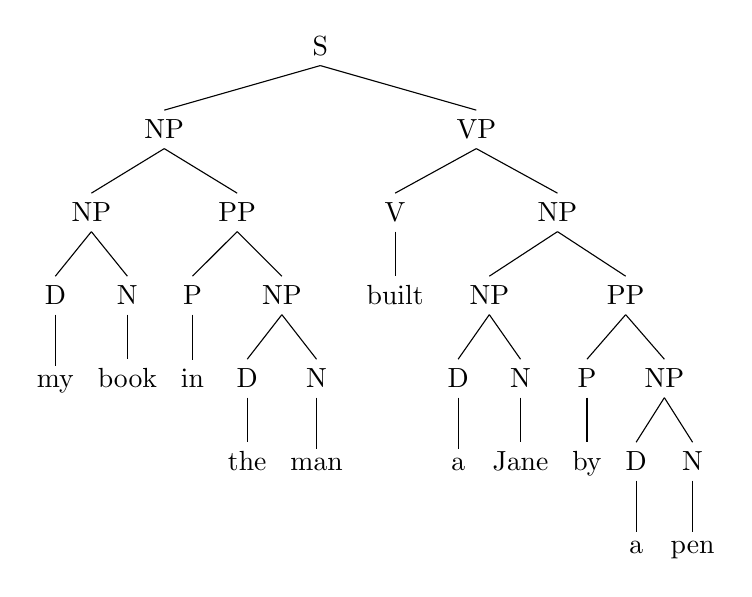
\begin{tikzpicture}[scale=1]
\Tree [.S [.NP [.NP [.D $$my$$ ] [.N $$book$$ ] ] [.PP [.P $$in$$ ] [.NP [.D $$the$$ ] [.N $$man$$ ]]] ][.VP [.V built ] [.NP [.NP [.D $$a$$ ] [.N $$Jane$$  ] ] [.PP [.P $$by$$ ] [.NP [.D $$a$$ ] [.N $$pen$$ ] ] ] ] ] ]
\end{tikzpicture}

\end{center}

\end{tcolorbox}

\newpage

Given the CFG below, answer \textbf{c}, \textbf{d} and \textbf{e} \\

\begin{lstlisting}[style=output,mathescape=true]
S  $\to$ E
E  $\to$ E + T | E - T | T
T  $\to$ T * I | T / I | I
I  $\to$ 0 | 1 | 2 | 3 | 4 | 6 | 7 | 8 | 9
\end{lstlisting}

\paragraph{c)} Provide the left-most derivation of 7 - 4 * 3 step-by-step and plot the final parse \hfill \small{(4/20 pts)} \\
tree matching that derivation \\

\begin{tcolorbox}
$S \xrightarrow{\text{L}} E$  $\xrightarrow{\text{L}} E-T$  $\xrightarrow{\text{L}} T-T$ $\xrightarrow{\text{L}} I-T$ $\xrightarrow{\text{L}} 7-T$  $\xrightarrow{\text{L}} 7-T*I$ $\xrightarrow{\text{L}} 7-I*I$ $\xrightarrow{\text{L}} 7-4*I$	$\xrightarrow{\text{L}} 7-4*3$

\end{tcolorbox}

\paragraph{d)} Provide the right-most derivation of 7 - 4 * 3 step-by-step and plot the final parse \hfill \small{(4/20 pts)} \\
 tree matching that derivation \\
 
\begin{tcolorbox}
$S \xrightarrow{\text{R}} E$  $\xrightarrow{\text{R}} E-T$  $\xrightarrow{\text{R}} E-T*I$ $\xrightarrow{\text{R}} E-T*3$ $\xrightarrow{\text{R}} E-I*3$  $\xrightarrow{\text{R}} E-4*3$ $\xrightarrow{\text{R}} T-4*3$ $\xrightarrow{\text{R}} I-4*3$ \\ 

$\xrightarrow{\text{R}} 7-4*3$

\end{tcolorbox}


\paragraph{e)} Are the derivations in \textbf{c} and \textbf{d} in the same similarity class?  \hfill \small{(4/20 pts)} \\

\begin{tcolorbox}
The leftmost derivation and rigthmost derivation of expression 7 - 4 * 3 are in the same similarity class.\\
Two derivations are similar if one of them can be transformed to other one by a sequence 'switching'.Such a switching can be applied to derivations which are related by precedence relation $\prec$.\\ 
Two derivation are related by $\prec$ if they are in the same reflexive,symmetric and transitive closure of $\prec$.\\
In this expression 7 - 4 * 3,let leftmost derivation is called as $D_1$ and rigthmost derivation is called as $D_n$.Since,two derivations are shown with the same parse tree,there exist $D_i$'s where $1<i<n$ and these $D_i$'s also are in the same similarity class.They make available such 'switchings' $D_1$ up to $D_n$.

\end{tcolorbox}


\newpage
\section{Pushdown Automata \hfill \normalfont{(30 pts)}}

\paragraph{a)} 
Find the language recognized by the PDA given below \hfill \small{(5/30 pts)} \\

\begin{tikzpicture}[shorten >=1pt,node distance=3cm,on grid,auto]
\node[state,initial,initial text=] (q_0) {$q_0$};
\node[state] (q_1) [right=of q_0] {$q_1$};
\node[state] (q_2) [above right=of q_1] {$q_2$};
\node[state] (q_3) [below right=of q_1] {$q_3$};
\node[state,accepting](q_4) [right=of q_2] {$q_4$};
\node[state](q_5) [right=of q_3] {$q_5$};
\node[state,accepting](q_6) [right=of q_5] {$q_6$};
\path[->]

(q_0) edge node {$\varepsilon,\varepsilon \to \#$} (q_1)
(q_1) edge [loop below] node {$x,\varepsilon \to x$} (q_1)

%%
(q_1) edge node {$\varepsilon,\varepsilon \to \varepsilon$} (q_2)
(q_2) edge [loop above] node {$y,x \to \varepsilon$} (q_2)

(q_2) edge node {$\varepsilon,\# \to \varepsilon$} (q_4)
(q_4) edge [loop above] node {$z,\varepsilon \to \varepsilon$} (q_4)

%%%

(q_1) edge node {$\varepsilon,\varepsilon \to \varepsilon$} (q_3)
(q_3) edge [loop below] node {$y,\varepsilon \to \varepsilon$} (q_3)

(q_3) edge node {$\varepsilon,\varepsilon \to \varepsilon$} (q_5)
(q_5) edge [loop below] node {$z,x \to \varepsilon$} (q_5)

(q_5) edge node {$\varepsilon,\# \to \varepsilon$} (q_6)
;
\end{tikzpicture} \\

\begin{minipage}{0.60\textwidth}
where the transition $((q_i,\alpha,\beta),(q_j,\gamma)) $ is represented as: 
\end{minipage}
\begin{minipage}{0.30\textwidth}
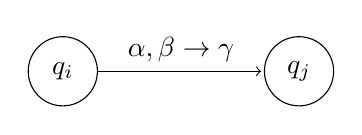
\begin{tikzpicture}[shorten >=1pt,node distance=3cm,on grid,auto]
\node[state] (q_i) {$q_i$};
\node[state] (q_j) [right=of q_i] {$q_j$};
\path[->]
(q_i) edge node {$\alpha,\beta \to \gamma$} (q_j);
\end{tikzpicture} \\
\end{minipage}


\begin{tcolorbox}

First,this automata pushes a \# in stack (and clearly it should be in bottom while other characters are pushing in stack).This \# will be used as end of the stack identifier.\\\\
After than,in $q_1$, $(x^*)$ is read.Now, there exist 2 choices.\\
1-Automata nondeteministically selects $q_2$ state.\\ 
2-Automata nondeteministically selects $q_3$ state.\\\\
In $q_2$ state,automata pops an 'x' for each read 'y'.At this step,there is no chance to read 'x','z' or 'y' more than number of read 'x'.When the only character in stack is '\#', automata nondeteministically goes to $q_4$ state by reading $\varepsilon$ and pops '\#' from stack.In $q_4$,$(z^*)$ is read. $q_4$ is a final state so if a string is read up to $q_4$,it is accepted by automata.\\
So,let the language accepted by upper part of automata ($q_2$ is picked) is $L_1$, then $L_1=\{x^ny^nz^m:n \geq 0,m \geq 0\}$.\\Also automata can pick $q_3$.\\
In $q_4$ state,$(y^*)$ is read and nothing is pushed to the stack.After reading y's, automata goes state $q_5$.In $q_5$ state,automata pops an 'x' for each read 'z'.At this step,there is no chance to read 'x','y' or 'z' more than number of read 'x'.When the only character in stack is '\#', automata nondeteministically goes to $q_6$ state by reading $\varepsilon$ and pops '\#' from stack. $q_6$ is a final state so if a string is read up to $q_6$,it is accepted by automata.\\
So,let the language accepted by lower part of automata ($q_3$ is picked) is $L_2$, then $L_2=\{x^ny^mz^n:n \geq 0,m \geq 0\}$.\\\\ 
Thus,the language recognized by the PDA is $L_1 \cup L_2$ which is $L_1 \cup L_2=L=\{\{x^ny^nz^m:n \geq 0,m \geq 0\} \cup \{x^ny^mz^n:n \geq 0,m \geq 0\}\}$.

\end{tcolorbox}

\newpage

\paragraph{b)} 
Design a PDA to recognize language $ L=\{x^n y^{m+n} x^m \mid \; n,m \geq 0; \; n,m \in \mathbb{N}  \} $  \hfill \small{(5/30 pts)} \\

\begin{tcolorbox}

\begin{center}
\begin{tikzpicture}[scale=0.2]
\tikzstyle{every node}+=[inner sep=0pt]
\draw [black] (11.5,-27.6) circle (3);
\draw (11.5,-27.6) node {$q_0$};
\draw [black] (24.6,-11.2) circle (3);
\draw (24.6,-11.2) node {$q_1$};
\draw [black] (46,-11.2) circle (3);
\draw (46,-11.2) node {$q_2$};
\draw [black] (61.4,-23.8) circle (3);
\draw (61.4,-23.8) node {$q_3$};
\draw [black] (46,-35.7) circle (3);
\draw (46,-35.7) node {$q_4$};
\draw [black] (26,-35.7) circle (3);
\draw (26,-35.7) node {$q_5$};
\draw [black] (26,-35.7) circle (2.4);
\draw [black] (48.32,-13.1) -- (59.08,-21.9);
\fill [black] (59.08,-21.9) -- (58.78,-21.01) -- (58.14,-21.78);
\draw (51.09,-17.99) node [below] {$\varepsilon,\#\to \#$};
\draw [black] (13.37,-25.26) -- (22.73,-13.54);
\fill [black] (22.73,-13.54) -- (21.84,-13.86) -- (22.62,-14.48);
\draw (18.61,-20.82) node [right] {$\varepsilon,\varepsilon\to \#$};
\draw [black] (22.219,-9.395) arc (260.56505:-27.43495:2.25);
\draw (18.91,-4.65) node [above] {$x,\varepsilon\to x$};
\fill [black] (24.58,-8.21) -- (25.21,-7.5) -- (24.22,-7.34);
\draw [black] (27.6,-11.2) -- (43,-11.2);
\fill [black] (43,-11.2) -- (42.2,-10.7) -- (42.2,-11.7);
\draw (35.3,-11.7) node [below] {$\varepsilon,\varepsilon\to \varepsilon$};
\draw [black] (46.96,-8.37) arc (189:-99:2.25);
\draw (51.3,-4.95) node [right] {$y,x\to \varepsilon$};
\fill [black] (48.83,-10.24) -- (49.7,-10.61) -- (49.54,-9.62);
\draw [black] (59.03,-25.63) -- (48.37,-33.87);
\fill [black] (48.37,-33.87) -- (49.31,-33.77) -- (48.7,-32.98);
\draw (51.09,-29.25) node [above] {$\varepsilon,\varepsilon\to \varepsilon$};
\draw [black] (63.768,-21.978) arc (155.30993:-132.69007:2.25);
\draw (68.76,-22.16) node [right] {$y,\varepsilon\to y$};
\fill [black] (64.29,-24.57) -- (64.81,-25.36) -- (65.22,-24.45);
\draw [black] (47.323,-38.38) arc (54:-234:2.25);
\draw (46,-42.95) node [below] {$x,y\to \varepsilon$};
\fill [black] (44.68,-38.38) -- (43.8,-38.73) -- (44.61,-39.32);
\draw [black] (43,-35.7) -- (29,-35.7);
\fill [black] (29,-35.7) -- (29.8,-36.2) -- (29.8,-35.2);
\draw (36,-35.2) node [above] {$\varepsilon,\#\to \varepsilon$};
\end{tikzpicture}
\end{center}

\end{tcolorbox}

\newpage

\paragraph{c)} 
Design a PDA to recognize language $ L=\{x^n y^m \mid \; n < m \leq 2n; \; n,m \in \mathbb{N^+} \} $  \hfill \small{(10/30 pts)} \\
Do not use multi-symbol push/pop operations in your transitions. \\
Simulate the PDA on strings \textit{xxy} (with only one rejecting derivation) and \textit{xxyyyy} (accepting derivation) with transition tables. \\


\begin{tcolorbox}

\begin{center}
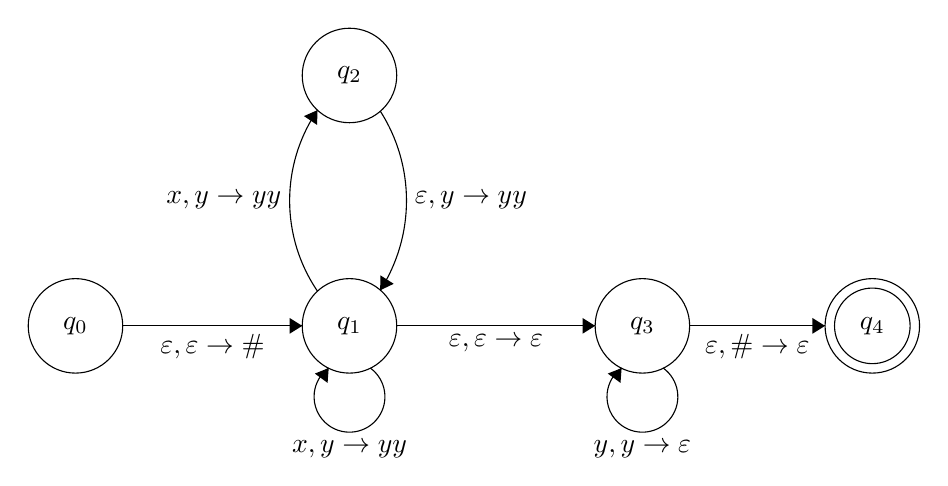
\begin{tikzpicture}[scale=0.2]
\tikzstyle{every node}+=[inner sep=0pt]
\draw [black] (14.4,-27.6) circle (3);
\draw (14.4,-27.6) node {$q_0$};
\draw [black] (31.8,-27.6) circle (3);
\draw (31.8,-27.6) node {$q_1$};
\draw [black] (31.8,-11.7) circle (3);
\draw (31.8,-11.7) node {$q_2$};
\draw [black] (50.4,-27.6) circle (3);
\draw (50.4,-27.6) node {$q_3$};
\draw [black] (65,-27.6) circle (3);
\draw (65,-27.6) node {$q_4$};
\draw [black] (65,-27.6) circle (2.4);
\draw [black] (17.4,-27.6) -- (28.8,-27.6);
\fill [black] (28.8,-27.6) -- (28,-27.1) -- (28,-28.1);
\draw (23.1,-28.1) node [below] {$\varepsilon,\varepsilon\to \#$};
\draw [black] (33.123,-30.28) arc (54:-234:2.25);
\draw (31.8,-34.85) node [below] {$x,y \to yy$};
\fill [black] (30.48,-30.28) -- (29.6,-30.63) -- (30.41,-31.22);
\draw [black] (29.773,-25.403) arc (-145.72083:-214.27917:10.214);
\fill [black] (29.77,-13.9) -- (28.91,-14.28) -- (29.74,-14.84);
\draw (27.5,-19.65) node [left] {$x,y \to yy$};
\draw [black] (51.723,-30.28) arc (54:-234:2.25);
\draw (50.4,-34.85) node [below] {$y,y \to \varepsilon$};
\fill [black] (49.08,-30.28) -- (48.2,-30.63) -- (49.01,-31.22);
\draw [black] (33.754,-13.963) arc (32.6558:-32.6558:10.54);
\fill [black] (33.75,-25.34) -- (34.61,-24.93) -- (33.76,-24.39);
\draw (35.92,-19.65) node [right] {$\varepsilon,y \to yy$};
\draw [black] (34.8,-27.6) -- (47.4,-27.6);
\fill [black] (47.4,-27.6) -- (46.6,-27.1) -- (46.6,-28.1);
\draw (41.1,-28.1) node [below] {$\varepsilon,\varepsilon\to \varepsilon$};
\draw [black] (53.4,-27.6) -- (62,-27.6);
\fill [black] (62,-27.6) -- (61.2,-27.1) -- (61.2,-28.1);
\draw (57.7,-28.1) node [below] {$\varepsilon,\# \to \varepsilon$};
\end{tikzpicture}
\end{center}

\vspace{19cm} % remove this after your answer
\end{tcolorbox}

\paragraph{d)} Given two languages $L'$ and $L$ as $L'=\{w \mid \; w\in L; \; |w|=4n+2 \; for\; n\in \mathbb{N} \}$
\hfill \small{(10/30 pts)} \\
If $L$ is a CFL, show that $L'$ is also a CFL by constructing an automaton for $L'$ in terms of another automaton that recognizes $L$. \\


\begin{tcolorbox}

Like the proof of how intersection of one Context Free Language and a regular language is another Context Free Language,another pushdown automaton can be constructed by taking the steps in the proof.\\\\
It is given that L is CFl,so there should be exist a PDA that rexognizes L.Let this PDA is called as $M_1$,then \\
$M_1=\{K_1,\Sigma_1,\Gamma_1,\Delta_1,S_1,F_1\}$  such that \\
$K_1$ is the finite set of states,\\
$\Sigma_1$ is input symbols,\\
$\Gamma_1$ is stack alphabet,\\
$\Delta_1$ is the transition rules,\\
$S_1 \in K_1$ is the initial state and\\
$F_1\subseteq K_1$ is the set of accepting states.\\\\
Now,suppose that language $L_1$ exists and $L_1=\{|w|=4n+2 \; for\; n\in \mathbb{N} \}$.This language is a regular language.Why this language is regular can be shown by creating a DFA.\\\\

\begin{center}
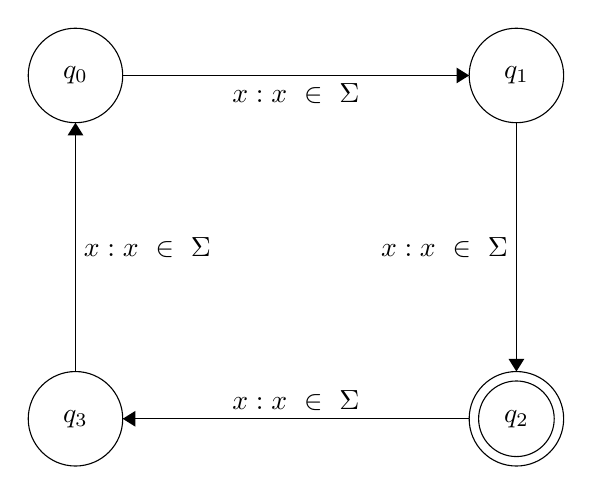
\begin{tikzpicture}[scale=0.2]
\tikzstyle{every node}+=[inner sep=0pt]
\draw [black] (19.3,-14.5) circle (3);
\draw (19.3,-14.5) node {$q_0$};
\draw [black] (47.3,-14.5) circle (3);
\draw (47.3,-14.5) node {$q_1$};
\draw [black] (47.3,-36.3) circle (3);
\draw (47.3,-36.3) node {$q_2$};
\draw [black] (47.3,-36.3) circle (2.4);
\draw [black] (19.3,-36.3) circle (3);
\draw (19.3,-36.3) node {$q_3$};
\draw [black] (22.3,-14.5) -- (44.3,-14.5);
\fill [black] (44.3,-14.5) -- (43.5,-14) -- (43.5,-15);
\draw (33.3,-15) node [below] {$x:x\mbox{ }\in\mbox{ }\Sigma$};
\draw [black] (47.3,-17.5) -- (47.3,-33.3);
\fill [black] (47.3,-33.3) -- (47.8,-32.5) -- (46.8,-32.5);
\draw (46.8,-25.4) node [left] {$x:x\mbox{ }\in\mbox{ }\Sigma$};
\draw [black] (44.3,-36.3) -- (22.3,-36.3);
\fill [black] (22.3,-36.3) -- (23.1,-36.8) -- (23.1,-35.8);
\draw (33.3,-35.8) node [above] {$x:x\mbox{ }\in\mbox{ }\Sigma$};
\draw [black] (19.3,-33.3) -- (19.3,-17.5);
\fill [black] (19.3,-17.5) -- (18.8,-18.3) -- (19.8,-18.3);
\draw (19.8,-25.4) node [right] {$x:x\mbox{ }\in\mbox{ }\Sigma$};
\end{tikzpicture}
\end{center}

Let this DFA called as $M_2$,then\\
$M_2=\{K_2,\Sigma_2,\delta_2,S_2,F_2\}$  such that \\
$K_2$ is the finite set of states,\\
$\Sigma_2$ is input symbols,\\
$\delta_2$ is the transition rules,\\
$S_2\in K_2$ is the initial state and\\
$F_2\subseteq K_2$ is the set of accepting states.\\\\

By closure property of intersection of a CFL and a regular language is a CFL as well, $L'$ is a CFL.Since every CFL is read by a PDA,there exist a PDA for $L'$.\\
Let the PDA for $L'$ called $M$, then $M$;\\
$M=(K,\Sigma_1,\Gamma,\Delta,S,F)$ where \\
$K=K_1\times K_2$\\
$\Gamma = \Gamma_1$\\
$S=(S_1,S_2)$ \\
$F = F_1 \times F_2$ and \\
$\Delta$ transition relation $=$ $(((q_1,q_2),\alpha,\beta),(p_1,p_2,\gamma))$ if and only if \\ both $((q_1,\alpha,\beta),(p_1,\gamma)) \in \Delta_1$  and $((q_2,\alpha),(p_1)) \in \delta_2$.\\
If pushdown automata has $\varepsilon$ transitions,\\
$\Delta$ transition relation $=$ $(((q_1,q_2),\varepsilon,\beta),(p_1,q_2,\gamma))$ if and only if\\
both $((q_1,\varepsilon,\beta),(p_1,\gamma)) \in \Delta_1$.\\Since,in every state,DFA accepts every character from alphabet,transitions in the DFA is not important,transitions  in $L'=L(M)$ come from the $L=L(M_1)$,however the important part of the DFA is it's accepting state.A word can be in $L=L(M_1)$ but if this word is not accepted by $L_1=L(M_2)$,then so does $L'=L(M)$.\\\\  
So,the costructed PDA $M$ is intersection of both $L=L(M_1)$ and $L_1=L(M_2)$ and  a word 'w' is in $L'=L(M)$ iff $w \in (L(M_1)\cap L(M_2))$.\\
   
\end{tcolorbox}

\newpage
\section{Closure Properties \hfill \normalfont{(20 pts)}}

Let $L_1$ and $L_2$ be context-free languages which are not regular, and let $L_3$ be a regular language. Determine whether the following languages are necessarily CFLs or not. If they need to be context-free, explain your reasoning. If not, give one example where the language is a CFL and a counter example where the language is not a CFL. \\

\paragraph{a)} $L_4 = L_1 \cap (L_2 \setminus L_3)$ \hfill \small{(10/20 pts)} \\

\begin{tcolorbox}
L4 is not necessarily be a Context Free Language.\\

$L2 \backslash {L3}$ $=$ $L2 \cap \bar{L3}$(by De Morgan's)\\
Since regular languages closed under comlementation,$\bar{L3}$ is a regular language as well.\\\\
Suppose that $L2=L(M_1)$ for a pushdown automaton ${M_1}=(K_1,\Sigma,\Gamma_1,\Delta_1,S_1,F_1)$ and $\bar{L3}=L(M_2)$ for a deterministic finite automaton(since every nondeterministic automata has an equal deterministic one,there should be exist a DFA to recognize this language) ${M_2}=(K_2,\Sigma,\delta_2,S_2,F_2)$.In order to prove that intersection of L2 and $\bar{L3}$ is context free as well,a new pushdown automata can be constructed.\\
Let $L2 \cap \bar{L3}=$ $L(M)$ and pushdown automata $M=(K,\Sigma,\Gamma,\Delta,S,F)$ where \\
$K=K_1\times K_2$\\
$\Gamma = \Gamma_1$\\
$S=(S_1,S_2)$ \\
$F = F_1 \times F_2$ and \\
$\Delta$ transition relation $=$ $(((q_1,q_2),\alpha,\beta),(p_1,p_2,\gamma))$ if and only if \\ both $((q_1,\alpha,\beta),(p_1,\gamma)) \in \Delta_1$  and $((q_2,\alpha),(p_1)) \in \delta_2$.\\
If pushdown automata has $\varepsilon$ transitions,\\
$\Delta$ transition relation $=$ $(((q_1,q_2),\varepsilon,\beta),(p_1,q_2,\gamma))$ if and only if\\
both $((q_1,\varepsilon,\beta),(p_1,\gamma)) \in \Delta_1$.\\
So,the a word 'w' is in L(M) iff $w \in (L(M_1)\cap L(M_2))$.\\
Thus, it is proved that $L2 \cap \bar{L3}$ is context free language.Let this language be 'L'.\\\\
Now,the question turns into whether $L_1 \cap L$ is context free or not.(Both languages are context free).In order to prove that intersection of 2 Context Free Language is not necessarily be CFL as well,a counter example can be given.\\Let $L1=\{a^nb^nc^m:n,m\geq0\}$ and $L=\{a^nb^mc^m:n,m\geq0\}$.(To show that these languages are context free,grammar for both can be given as:\\Rules for L1:$S\to S1S2;S1\to aS1b|\varepsilon;S2\to cS2|\varepsilon$,\\Rules for L:$S\to S1S2;S1\to aS1|\varepsilon;S2\to bS2c|\varepsilon$).\\
$L1\cap L=\{a^nb^nc^n:n\geq0\}$.Assume that $L1\cap L$ is CFL and $w \in L1\cap L$.(length of w$=|w|>\phi(G)^{|V-\Sigma|}$ )\\By pumping lemma,this word w can be split into 5 part namely u,v,x,y,z.Then there exist an integer k and $k>(\frac{\phi(G)^{|V-\Sigma|}}{3}$) such that
$w=a^kb^kc^k$,clearly,$k<|w|$.\\And there exist a split such that:\\
$w=uvxyz$, $|vxy|\leq k$ and $|vy|\geq 1$.Then,$w=uv^ixy^iz$ should be hold for every $i\geq 0$.\\5 possible partitions are:\\
1-vxy part consist of all a's ;2-vxy part consist of all b's;3-vxy part consist of all c's;4-vxy part consist of a's and b's;5-vxy part consist of  b's and c's.\\
In first 3,if i is chosen as 0,the word becomes $w=a^{k-l}b^kc^k$ or $w=a^kb^{k-l}c^k$ or $w=a^kb^kc^{k-l}$ respectively and $w\notin$ $L1\cap L$.(l is the total length of v and y parts)\\ 
İn last 2 possibilities,if i is chosen as 0,the word w becomes $w=a^{k-l}b^{k-l}c^k$ or $w=a^kb^{k-l}c^{k-l}$ and clearly both generated $w\notin$
$L1\cap L$.(l is the total length of v and y parts)\\
Thus,by using pumping lemma,the language $L1\cap L=\{a^nb^nc^n:n\geq0\}$ is not a Context Free Language.\\\\
In a nutshell,firstly is is proved that $L2 \backslash {L3}$ is a context free language by using De Morgan Laws and constructing a pushdown automata for it.Afterwards,it is demonstrated that intersection of 2 context free language is not necessarily a Context Free Language.In order to show this,pumping lemma for CFL and counter example are used.\\

L4 is not necessarily be a Context Free Language.\\ 
 
\end{tcolorbox}

\paragraph{b)} $L_5 = (L_1 \cap L_3)\text{*}$ \hfill \small{(10/20 pts)} \\

\begin{tcolorbox}

L5 is necessarily be a Context Free Language.\\

First $L1 \cap \L3$ should be analyzed.
Suppose that $L1=L(M_1)$ for a pushdown automaton ${M_1}=(K_1,\Sigma,\Gamma_1,\Delta_1,S_1,F_1)$ and $L3=L(M_2)$ for a deterministic finite automaton(since every nondeterministic automata has an equal deterministic one,there should be exist a DFA to recognize this language) ${M_2}=(K_2,\Sigma,\delta_2,S_2,F_2)$.In order to prove that intersection of $L1$ and $L3$ is context free as well,a new pushdown automata can be constructed.\\
Let $L1 \cap L3=$ $L(M)$ and pushdown automata $M=(K,\Sigma,\Gamma,\Delta,S,F)$ where \\
$K=K_1\times K_2$\\
$\Gamma = \Gamma_1$\\
$S=(S_1,S_2)$ \\
$F = F_1 \times F_2$ and \\
$\Delta$ transition relation $=$ $(((q_1,q_2),\alpha,\beta),(p_1,p_2,\gamma))$ if and only if \\ both $((q_1,\alpha,\beta),(p_1,\gamma)) \in \Delta_1$  and $((q_2,\alpha),(p_1)) \in \delta_2$.\\
If pushdown automata has $\varepsilon$ transitions,\\
$\Delta$ transition relation $=$ $(((q_1,q_2),\varepsilon,\beta),(p_1,q_2,\gamma))$ if and only if\\
both $((q_1,\varepsilon,\beta),(p_1,\gamma)) \in \Delta_1$.\\
So,the a word 'w' is in L(M) iff $w \in (L(M_1)\cap L(M_2))$.\\
Thus, it is proved that $L1 \cap L3$ is context free language.Let this language be 'L'.\\\\
Now,the question becomes whether $L_5 = (L_1 \cap L_3)\text{*}$ $=L^*$ is context free language or not.It is known that L is CFL.By using closure property of CFL under 'kleene star',it can be proved that $L^*$ is CFL.\\ 
Let language L is generated by grammar G,namely $L=L(G)$ and $G=\{V,\Sigma,R,S\}$.\\
A new grammar $G_1$ for $L^*$ can be written by using grammar G.\\
$L^*=L(G_1)$ and $G_1=\{V\cup \{S_1\},\Sigma,R\cup \{S_1 \to \varepsilon,S_1 \to S_1S\},S_1\}$.
What we have done to obtain $G_1$ are:\\ -adding a new starting point to $G$ and adding rule $\{S_1 \to \varepsilon\}$.By this rule,this grammar can create a word $\{\}$ like 'kleene star';\\-also add the rule $\{S_1 \to S_1S\}$ for creating a word as many long as we want by using the rules in grammar $G$ (so does 'kleene star').\\\\
To sum up,firstly, it is demonstrated that $L1 \cap \L3$ is Context Free Language by constructing a pushdown automata to recognize the language $L1 \cap \L3$.Afterwards,by using Context Free Languages are closed under 'kleene star' property,it is proved that $L_5 = (L_1 \cap L_3)\text{*}$ is      
 Context Free Language as well.\\\\
 Thus, $L_5 = (L_1 \cap L_3)\text{*}$ is necessarily be a CFL.\\

\end{tcolorbox}





\newpage
\section{Pumping Theorem \hfill \normalfont{(20 pts)}}

\paragraph{a)} Show that $L=\{a^n m^n t^i \mid \; n\leq i \leq 2n\}$ is not a Context Free Language \hfill \small{(10/20 pts)} \\
using Pumping Theorem for CFLs. \\

\begin{tcolorbox}

$L=\{a^n m^n t^i \mid \; n\leq i \leq 2n\}$ is not a Context Free Language.\\\\

Assume that $L$ is a CFL and $w$ is a word $\in L$.(length of w $=|w|>\phi(G)^{|V-\Sigma|}$ )\\By pumping lemma,this word w can be split into 5 part namely u,v,x,y,z.Then there exist an integer k such that
$w=a^km^kt^i$,clearly,$k<|w|$.\\And there exist a split such that:\\
$w=uvxyz$, $|vxy|\leq k$ and $|vy|\geq 1$.Then,$w=uv^jxy^jz$ should be hold for every $j\geq 0$.\\5 possible partitions are:\\\\
1-vxy part consist of all a's:\\\\
Then,$u=a^l$, $v=a^p$,$x=a^r$, $y=a^s$ and $z=a^hm^kt^i$ such that:\\
$l+p+r+s+h=k$,$p+r+s\leq k$ and $p+s\geq 1$.\\
Pumping lemma states that $w=uv^jxy^jz$ should be hold for every $j\geq 0$.\\
Let j is taken as 0.Then,$u=a^l$, $v={(a^p)}^0=0$,$x=a^r$, $y={(a^s)}^0=0$ and $z=a^hm^kt^i$.\\The word w becomes $w=a^{k-p-s}m^kt^i$.It is clear that number of a's in this word is not equal to number of m's.So,new $w \notin L$.\\  

2-vxy part consist of all m's;\\\\
Then,$u=a^km^h$, $v=m^p$,$x=m^r$, $y=m^s$ and $z=m^lt^i$ such that:\\
$l+p+r+s+h=k$,$p+r+s\leq k$ and $p+s\geq 1$.\\
Pumping lemma states that $w=uv^jxy^jz$ should be hold for every $j\geq 0$.\\
Let j is taken as 0.Then,$u=a^km^h$, $v={(m^p)}^0=0$,$x=m^r$, $y={(m^s)}^0=0$ and $z=t^i$.\\The word w becomes $w=a^km^{k-p-s}t^i$.It is clear that number of a's in this word is not equal to number of m's.So,new $w \notin L$.\\

3-vxy part consist of all t's;\\\\
Then,$u=a^km^kt^h$, $v=t^l$,$x=t^p$, $y=t^r$ and $z=t^s$ such that:\\
$l+p+r+s+h=i$ and $l+r\geq 1$.\\
Pumping lemma states that $w=uv^jxy^j$ should be hold for every $j\geq 0$.\\
Let j is taken as $(2\times n+1)$.Then,$u=a^km^kt^h$, $v={(t^l)}^{2n+1}$,$x=t^p$, $y={(t^r)}^{2n+1}$ and $z=t^s$.\\The word w becomes $w=a^km^kt^{i+(l\times 2n)+(r\times 2n)}$.Since i at least as big as n ($n\leq i$) and at least one of $t^l$ or $t^r$ part is not empty,namely$(|l|+|r|)\geq 1$,the pumped w has at least i+2n t's in it.This is unsuitable because there is a given constraint that i should less than 2n. So,new $w \notin L$.\\

4-v and y part consist of same number of a's and m's respectively;\\\\
Firstly,in $w=uvxyz$, it is clear that if v and y part has unequal number of a and m's,the generated word w after pumping does not have equal number of a's and m's in it.This is clearly not in language L.\\
If v and y part consist of same number of a's and m's,then for any $j\geq i$,since v and y parts cannot be empty at the same time,namely$(|l|+|r|)\geq 1$,the 'pumped' word definitely have more a's and m's than t's in it.However,this is against to constraint $n\leq i$.Thus,there is no chance to $w\in L$.\\

5-v part includes m's and y part includes t's;\\\\
There are 3 possibilities as well in such a split,which are $|v|=|y|$, $|v|\leq |y|$ and $|v|\geq |y|$.\\\\ 
If $|v|=|y|$,that is if number of m's in v part equal to number of t's in y part,$n\leq i$ constraint is conserved and number of a's and number of m's in w are less than number of t's.Although  $n\leq i$ is conserved,then number of a's and number of m's are not equal to each other.\\
If $|v|\leq |y|$, both number of a's and number of m's are not equal to each other in w and for big j's(pumping number),unfortunately i will pass 2n.\\
If $|v|\geq |y|$, both number of a's and number of m's are not equal to each other in w and for big j's(pumping number),unfortunately n will pass i.\\
Thus,there is no chance to $w\in L$.\\\\

The only solution which does not harm the constraints ($n\leq i \leq 2n$) and number of a's and m's should be equal in w, is like that:\\
$w=uvxyz$, v part consist of same number of a and m's and y part has the same length of v part.\\However,in such split length of vxy part exceeds the limit.To put a finer point on it,as I mentioned at the top,there exist an integer k which should be  greater than $|vxy|$ part.\\\\

Thus,there is no split ends up with a word which is in language and does not damage the constraints.At the top,it is assumed that this language L is a CFL but by pumping lemma, it was shown  that all possible parititons lead to contradiction.So,L is not a CFL.\\     

\end{tcolorbox}

\newpage

\paragraph{b)} Show that $L=\{a^n b^{2n} a^n \mid \; n \in \mathbb{N+} \}$ is not a Context Free Language \hfill \small{(10/20 pts)} \\
using Pumping Theorem for CFLs. \\


\begin{tcolorbox}

$L=\{a^n b^{2n} a^n \mid \; n \in \mathbb{N+} \}$ is not a Context Free Language.\\\\
Assume that $L$ is a CFL and $w$ is a word $\in L$.(length of w $=|w|>\phi(G)^{|V-\Sigma|}$ )\\By pumping lemma,this word w can be split into 5 part namely u,v,x,y,z.Then there exist an integer k and  such that
$w=a^kb^{2k}a^k$,clearly,$k<|w|$.\\And there exist a split such that:\\
$w=uvxyz$, $|vxy|\leq k$ and $|vy|\geq 1$.Then,$w=uv^jxy^jz$ should be hold for every $j\geq 0$.\\5 possible partitions are:\\\\
1-vxy part consist of first group a's:\\\\
Then,$u=a^l$, $v=a^p$,$x=a^r$, $y=a^s$ and $z=a^hb^{2k}a^k$ such that:\\
$l+p+r+s+h=k$,$p+r+s\leq k$ and $p+s\geq 1$.\\
Pumping lemma states that $w=uv^jxy^jz$ should be hold for every $j\geq 0$.\\
Let j is taken as 0.Then,$u=a^l$, $v={(a^p)}^0=0$,$x=a^r$, $y={(a^s)}^0=0$ and $z=a^hb^{2k}a^k$.\\The word w becomes $w=a^{k-p-s}b^{2k}a^k$.It is clear that number of a's before b's in this word is not equal to number of a's after b's.So,new $w \notin L$.\\  

2-vxy part consist of b's;\\\\
Then,$u=a^kb^l$, $v=b^p$,$x=b^r$, $y=b^s$ and $z=b^ha^k$ such that:\\
$p+r+s+l+h=2k$,$p+r+s\leq k$ and $p+s\geq 1$.\\
Pumping lemma states that $w=uv^jxy^jz$ should be hold for every $j\geq 0$.\\
Let j is taken as 0.Then,$u=a^kb^l$, $v={(b^p)}^0=0$,$x=b^r$, $y={(b^s)}^0=0$ and $z=b^ha^k$.\\The word w becomes $w=a^kb^{2k-p-s}a^k$.It is clear that total number of a's in this word is not equal to number of b's.So,new $w \notin L$.\\

3-vxy part consist of second group a's;\\\\
Then,$u=a^kb^{2k}a^h$, $v=a^l$,$x=a^p$, $y=a^r$ and $z=a^s$ such that:\\
$h+l+p+r+s=i$, $l+p+r\leq k$ and $l+r\geq 1$.\\
Pumping lemma states that $w=uv^jxy^j$ should be hold for every $j\geq 0$.\\
Let j is taken as 0.Then,$u=a^kb^{2k}a^h$, $v={(a^l)}^0=0$,$x=a^p$, $y={(a^r)}^0=0$ and $z=a^s$.\\The word w becomes $w=a^kb^{2k}a^{k-l-r}$.It is clear that number of a's after b's in this word is not equal to number of a's before b's.So,new $w \notin L$.\\

4-v part includes a's and y part includes b's with length $2\times |v|$;\\\\
Firstly,in $w=uvxyz$, it is clear that if v and y part don't have this fraction,the generated word w after pumping does not conserve number of a's before b's is half of b's in it.This is clearly not in language L.\\
If v and y part consist of  a's and b's respectively with y part's length is 2 times of v,then for any $j\geq i$,since v and y parts cannot be empty at the same time,namely$(|l|+|r|)\geq 1$,the 'pumped' word definitely have more a's before b's than a's after b's in it.However,this is against to constraint that number of a's in two end in the word is same.Thus,there is no chance to $w\in L$.\\

5-v part includes b's with length $2\times |y|$ and y part includes a's ;\\\\
Firstly,in $w=uvxyz$, it is clear that if v and y part don't have this fraction,the generated word w after pumping does not conserve number of a's after b's is half of b's in it.This is clearly not in language L.\\
If v and y part consist of  b's and a's respectively with v part's length is 2 times of y,then for any $j\geq i$,since v and y parts cannot be empty at the same time,namely$(|l|+|r|)\geq 1$,the 'pumped' word definitely have more a's after b's than a's before b's in it.However,this is against to constraint that number of a's in two end in the word is same.Thus,there is no chance to $w\in L$.\\



The only solution which does not harm the constraints total number of b's and a's are equal and number of a's at the two end of word should be equal in w, is like that:\\
$w=uvxyz$, v part consist of a and b's where number of b's is 2 times of a's and y part has the same property of v part.(begin b's and after a's,number of b's is 2 times of number of a's)\\However,in such split length of vxy part exceeds the limit.To put a finer point on it,as I mentioned at the top,there exist an integer k which should be  greater than $|vxy|$ part but in this split whole b's in $vxy$ part and also there exist a's in this part.$2k$ cannot be less than $vxy$ part.\\\\

Thus,there is no split ends up with a word which is in language and does not damage the constraints.At the top,it is assumed that this language L is a CFL but by pumping lemma, it was shown  that all possible parititons lead to contradiction.So,L is not a CFL.\\

\end{tcolorbox}


\newpage
\section{CNF and CYK \hfill \normalfont{(not graded)}}

\paragraph{a)} Convert the given context-free grammar to Chomsky Normal Form. \\

$ S   \to XSX \mid xY $ \\
$ X   \to Y \mid S $ \\
$ Y   \to z \mid \varepsilon $ \\

\begin{tcolorbox}
answer here ...
\vspace{18cm} % remove this after your answer
\end{tcolorbox}


\paragraph{b)} Use the grammar below to parse the given sentence using Cocke–Younger–Kasami algorithm. \\
Plot the parse trees. \\

\begin{multicols}{2}
S $\to$ NP VP \\
S $\to$ X1 VP \\
X1 $\to$ Aux NP \\
S $\to$ book $\mid$ include $\mid$ prefer \\
S $\to$ Verb NP \\
S $\to$ X2 PP \\
S $\to$ Verb PP \\
S $\to$ VP PP \\
NP $\to$ I $\mid$ she $\mid$ me $\mid$ Houston \\
NP $\to$ Det Nom \\
Nom $\to$ book $\mid$ flight $\mid$ meal $\mid$ money \\
Nom $\to$ Nom Noun \\
Nom $\to$ Nom PP \\
VP $\to$ book $\mid$ include $\mid$ prefer \\
VP $\to$ Verb NP \\
VP $\to$ X2 PP \\
X2 $\to$ Verb NP \\
VP $\to$ Verb PP \\
VP $\to$ VP PP \\
PP $\to$ Prep NP \\
Det $\to$ that $\mid$ this $\mid$ the $\mid$ a \\
Noun $\to$ book $\mid$ flight $\mid$ meal $\mid$ money \\
Verb $\to$ book $\mid$ include $\mid$ prefer \\
Aux $\to$ does \\
Prep $\to$ from $\mid$ to $\mid$ on $\mid$ near $\mid$ through \\
\end{multicols}

\vspace{5mm}

book the flight through Houston \\

\begin{tcolorbox}

\scriptsize

Empty parse table:\\
\begin{tikzpicture}[node distance=0cm, outer sep = 0pt]

\node[terminal] (l0) {
    \begin{tabular}{@{}P{2.9cm}|@{}P{2.9cm}|@{}P{2.9cm}|@{}P{2.9cm}|@{}P{2.9cm}}
    book & the & flight & through & Houston \\
    \end{tabular}
};

\node[nonterminal] (l1) [above = of l0] {
    \begin{tabular}{@{}P{2.9cm}|@{}P{2.9cm}|@{}P{2.9cm}|@{}P{2.9cm}|@{}P{2.9cm}}
    1:1 & 
    2:2 & 
    3:3 & 
    4:4 & 
    5:5 \\
    \end{tabular}
};

\node[nonterminal] (l2) [above = of l1.north] {
    \begin{tabular}{@{}P{2.9cm}|@{}P{2.9cm}|@{}P{2.9cm}|@{}P{2.9cm}}
    1:2 $\to$ 1:1 2:2 & 
    2:3 $\to$ 2:2 3:3 & 
    3:4 $\to$ 3:3 4:4 & 
    4:5 $\to$ 4:4 5:5 \\
    \end{tabular}
};

\node[nonterminal] (l3) [above = of l2.north] {
    \begin{tabular}{@{}P{2.9cm}|@{}P{2.9cm}|@{}P{2.9cm}}
        \begin{tabular}{@{}l} 1:3 $\to$ 1:1 2:3 \\ 1:3 $\to$ 1:2 3:3 \end{tabular}& 
        \begin{tabular}{@{}l} 2:4 $\to$ 2:2 3:4 \\ 2:4 $\to$ 2:3 4:4 \end{tabular}& 
        \begin{tabular}{@{}l} 3:5 $\to$ 3:3 4:5 \\ 3:5 $\to$ 3:4 5:5 \end{tabular}\\
    \end{tabular}
};

\node[nonterminal] (l4) [above = of l3.north] {
    \begin{tabular}{@{}P{2.9cm}|@{}P{2.9cm}}
        \begin{tabular}{@{}l}1:4 $\to$ 1:1 2:4 \\ 1:4 $\to$ 1:2 3:4 \\ 1:4 $\to$ 1:3 4:4 \end{tabular}& 
        \begin{tabular}{@{}l}2:5 $\to$ 2:2 3:5 \\ 2:5 $\to$ 2:3 4:5 \\ 2:5 $\to$ 2:4 5:5 \end{tabular}\\
    \end{tabular}
};

\node[nonterminal] (l5) [above = of l4.north] {
    \begin{tabular}{@{}P{2.9cm}}
        \begin{tabular}{@{}l}
        1:5 $\to$ 1:1 2:5 \\ 1:5 $\to$ 1:2 3:5 \\ 
        1:5 $\to$ 1:3 4:5 \\ 1:5 $\to$ 1:4 5:5 
        \end{tabular}\\
    \end{tabular}
};

\end{tikzpicture}\\\\

rest of the answer here ...\\
\vspace{4cm} % remove this after your answer
\end{tcolorbox}



\newpage
\section{Deterministic Pushdown Automata \hfill \normalfont{(not graded)}}
Provide a DPDA to recognize the given languages, the DPDA must read its entire input and finish with an empty stack.
\paragraph{a)} $a^*bc \cup a^nb^nc$ \\

\begin{tcolorbox}
answer here ...
\vspace{12cm} % remove this after your answer
\end{tcolorbox}

\newpage

\paragraph{b)} $(aa)^*c \cup a^nb^nc$ \\

\begin{tcolorbox}
answer here ...
\vspace{12cm} % remove this after your answer
\end{tcolorbox}



\end{document}

​
